\section{Resolved stellar mass-to-light ratios: Discussion and Conclusion}
\label{chap1:sec:discussion}

In this work, we construct a set of \nSFHs synthetic SFHs (subsampled \nsubsample times in ${\rm [Z]}$, $\tau_V$, $\mu$, and $\sigma$), perform PCA on the resulting optical spectra, and use the resulting, lower-dimensional space to fit IFS observations from the SDSS-IV/MaNGA survey. Using those fits, we estimate resolved, $i$-band stellar mass-to-light ratios for galaxies in \mplv, with uncertainties which take into account model-dependent and age-metallicity degeneracies, as well as a spectrophotometric covariance estimated from multiply-observed galaxies. The parameter-estimation strategy chosen performs well when tested on synthetic, test data generated identically to the training data, at median signal-to-noise ratios between 2 and 20 (see Figures \ref{fig:mocks_snr_color_hist_devMLi}, \ref{fig:mocks_snr_color_hist_widMLi}, and \ref{fig:mocks_snr_color_hist_devwidMLi}). We note that deviations in this intermediate-signal-to-noise regime generally lie at the $\sim 0.1$ dex level or smaller, and are mostly uncorrelated with stellar metallicity and foreground attenuation. At higher and lower median signal-to-noise, extreme values of these two parameters correlate with mis-estimates of $\Upsilon^*_i$ at the $\sim 0.2$ dex level.

We include here sample maps of resolved stellar mass-to-light ratio for a sample of three early-type galaxies (Figure \ref{fig:ETG_montage}) and four late-type galaxies (Figure \ref{fig:LTG_montage}), including uncertainties \& data-quality masks, accompanied by a cutout image of the galaxy from legacy imaging.
%
\begin{figure*}
    \centering
    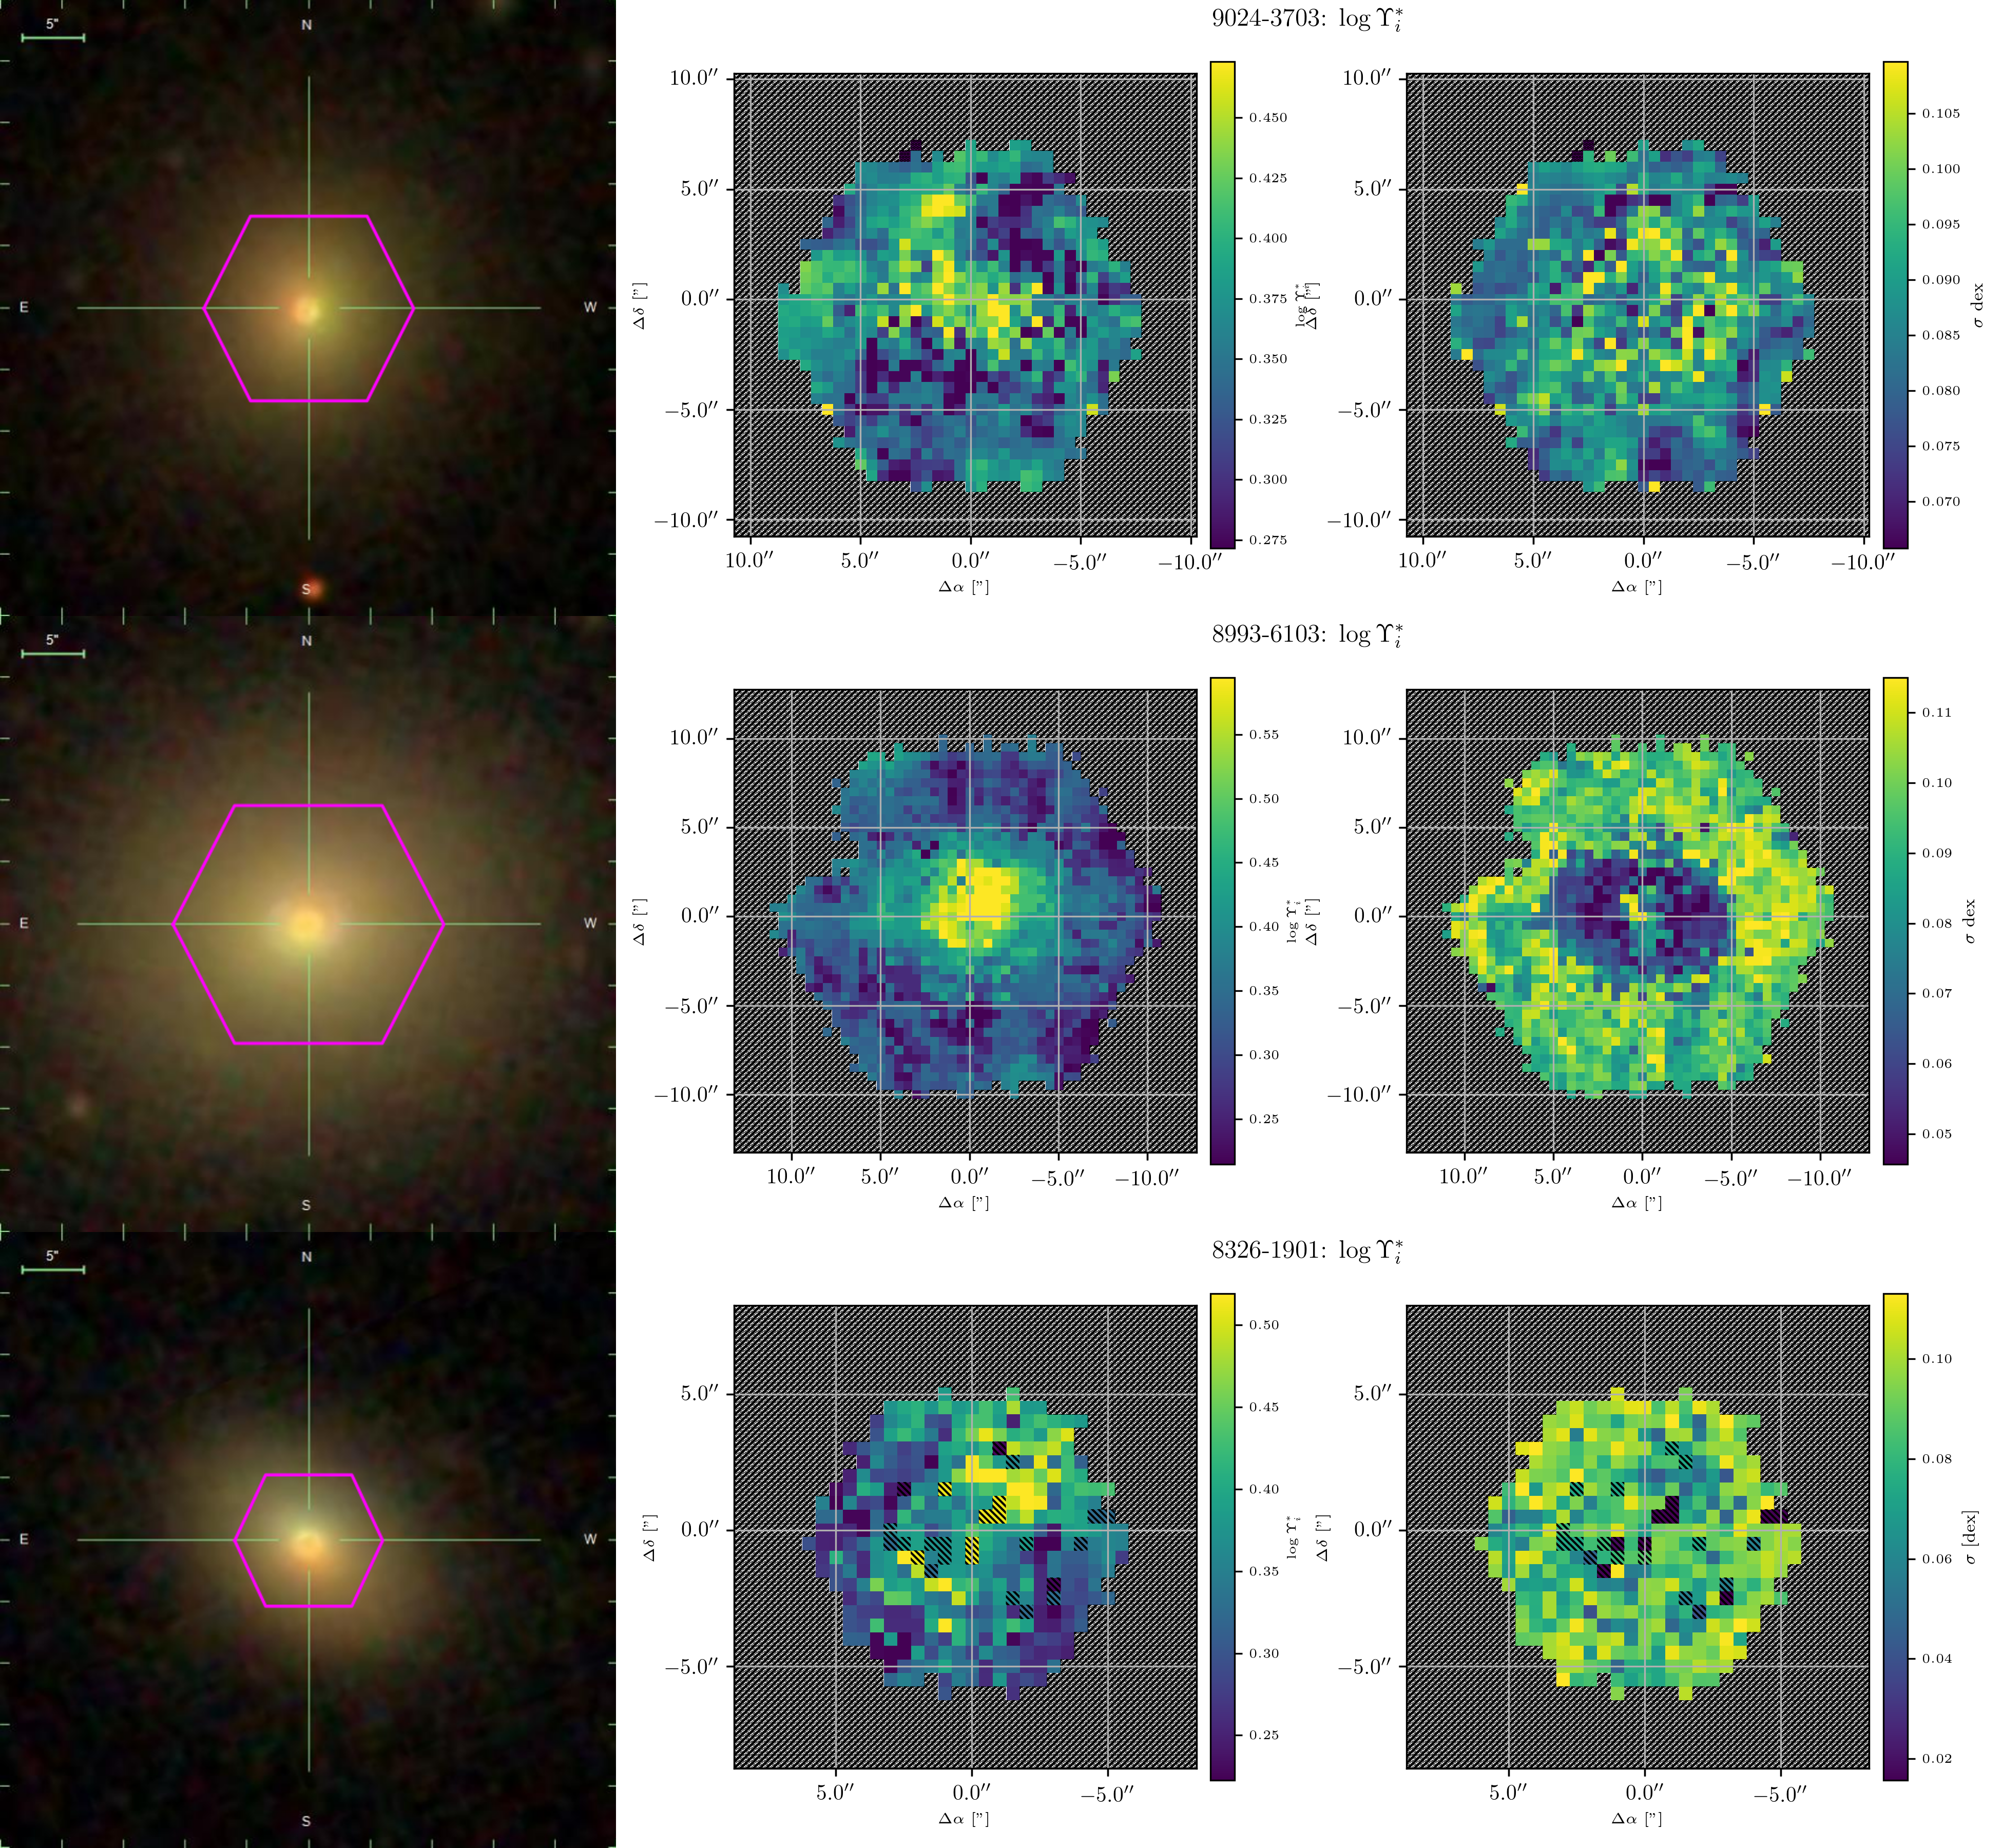
\includegraphics[width=0.95\textwidth]{ETG_montage}
    \caption[Maps of $i$-band stellar mass-to-light ratio for three early-type galaxies]{\fixspacing A selection of three early-type galaxies: In the left-hand column, the SDSS cutout with a purple hexagon denoting the approximate spatial grasp of the IFU. In the middle column, an image of the resolved estimate of $i$-band stellar mass-to-light ratio, taken as the 50$^{\rm th}$ percentile of the posterior PDF for a given spaxel. In the right-hand panel, a map of the adopted uncertainty in stellar mass-to-light ratio, taken as half the difference between the 16$^{\rm th}$ and 84$^{\rm th}$ percentiles of the posterior PDF. Spaxels with hatching top-left to bottom-right have poorly-sampled PDFs, and spaxels with hatching top-right to bottom-left have no data. Spaxels filled with dots had a numerical failure in the PC down-projection, which prevented an estimate from being made (very rare).}
    \label{fig:ETG_montage}
\end{figure*}
%
\begin{figure*}
    \centering
    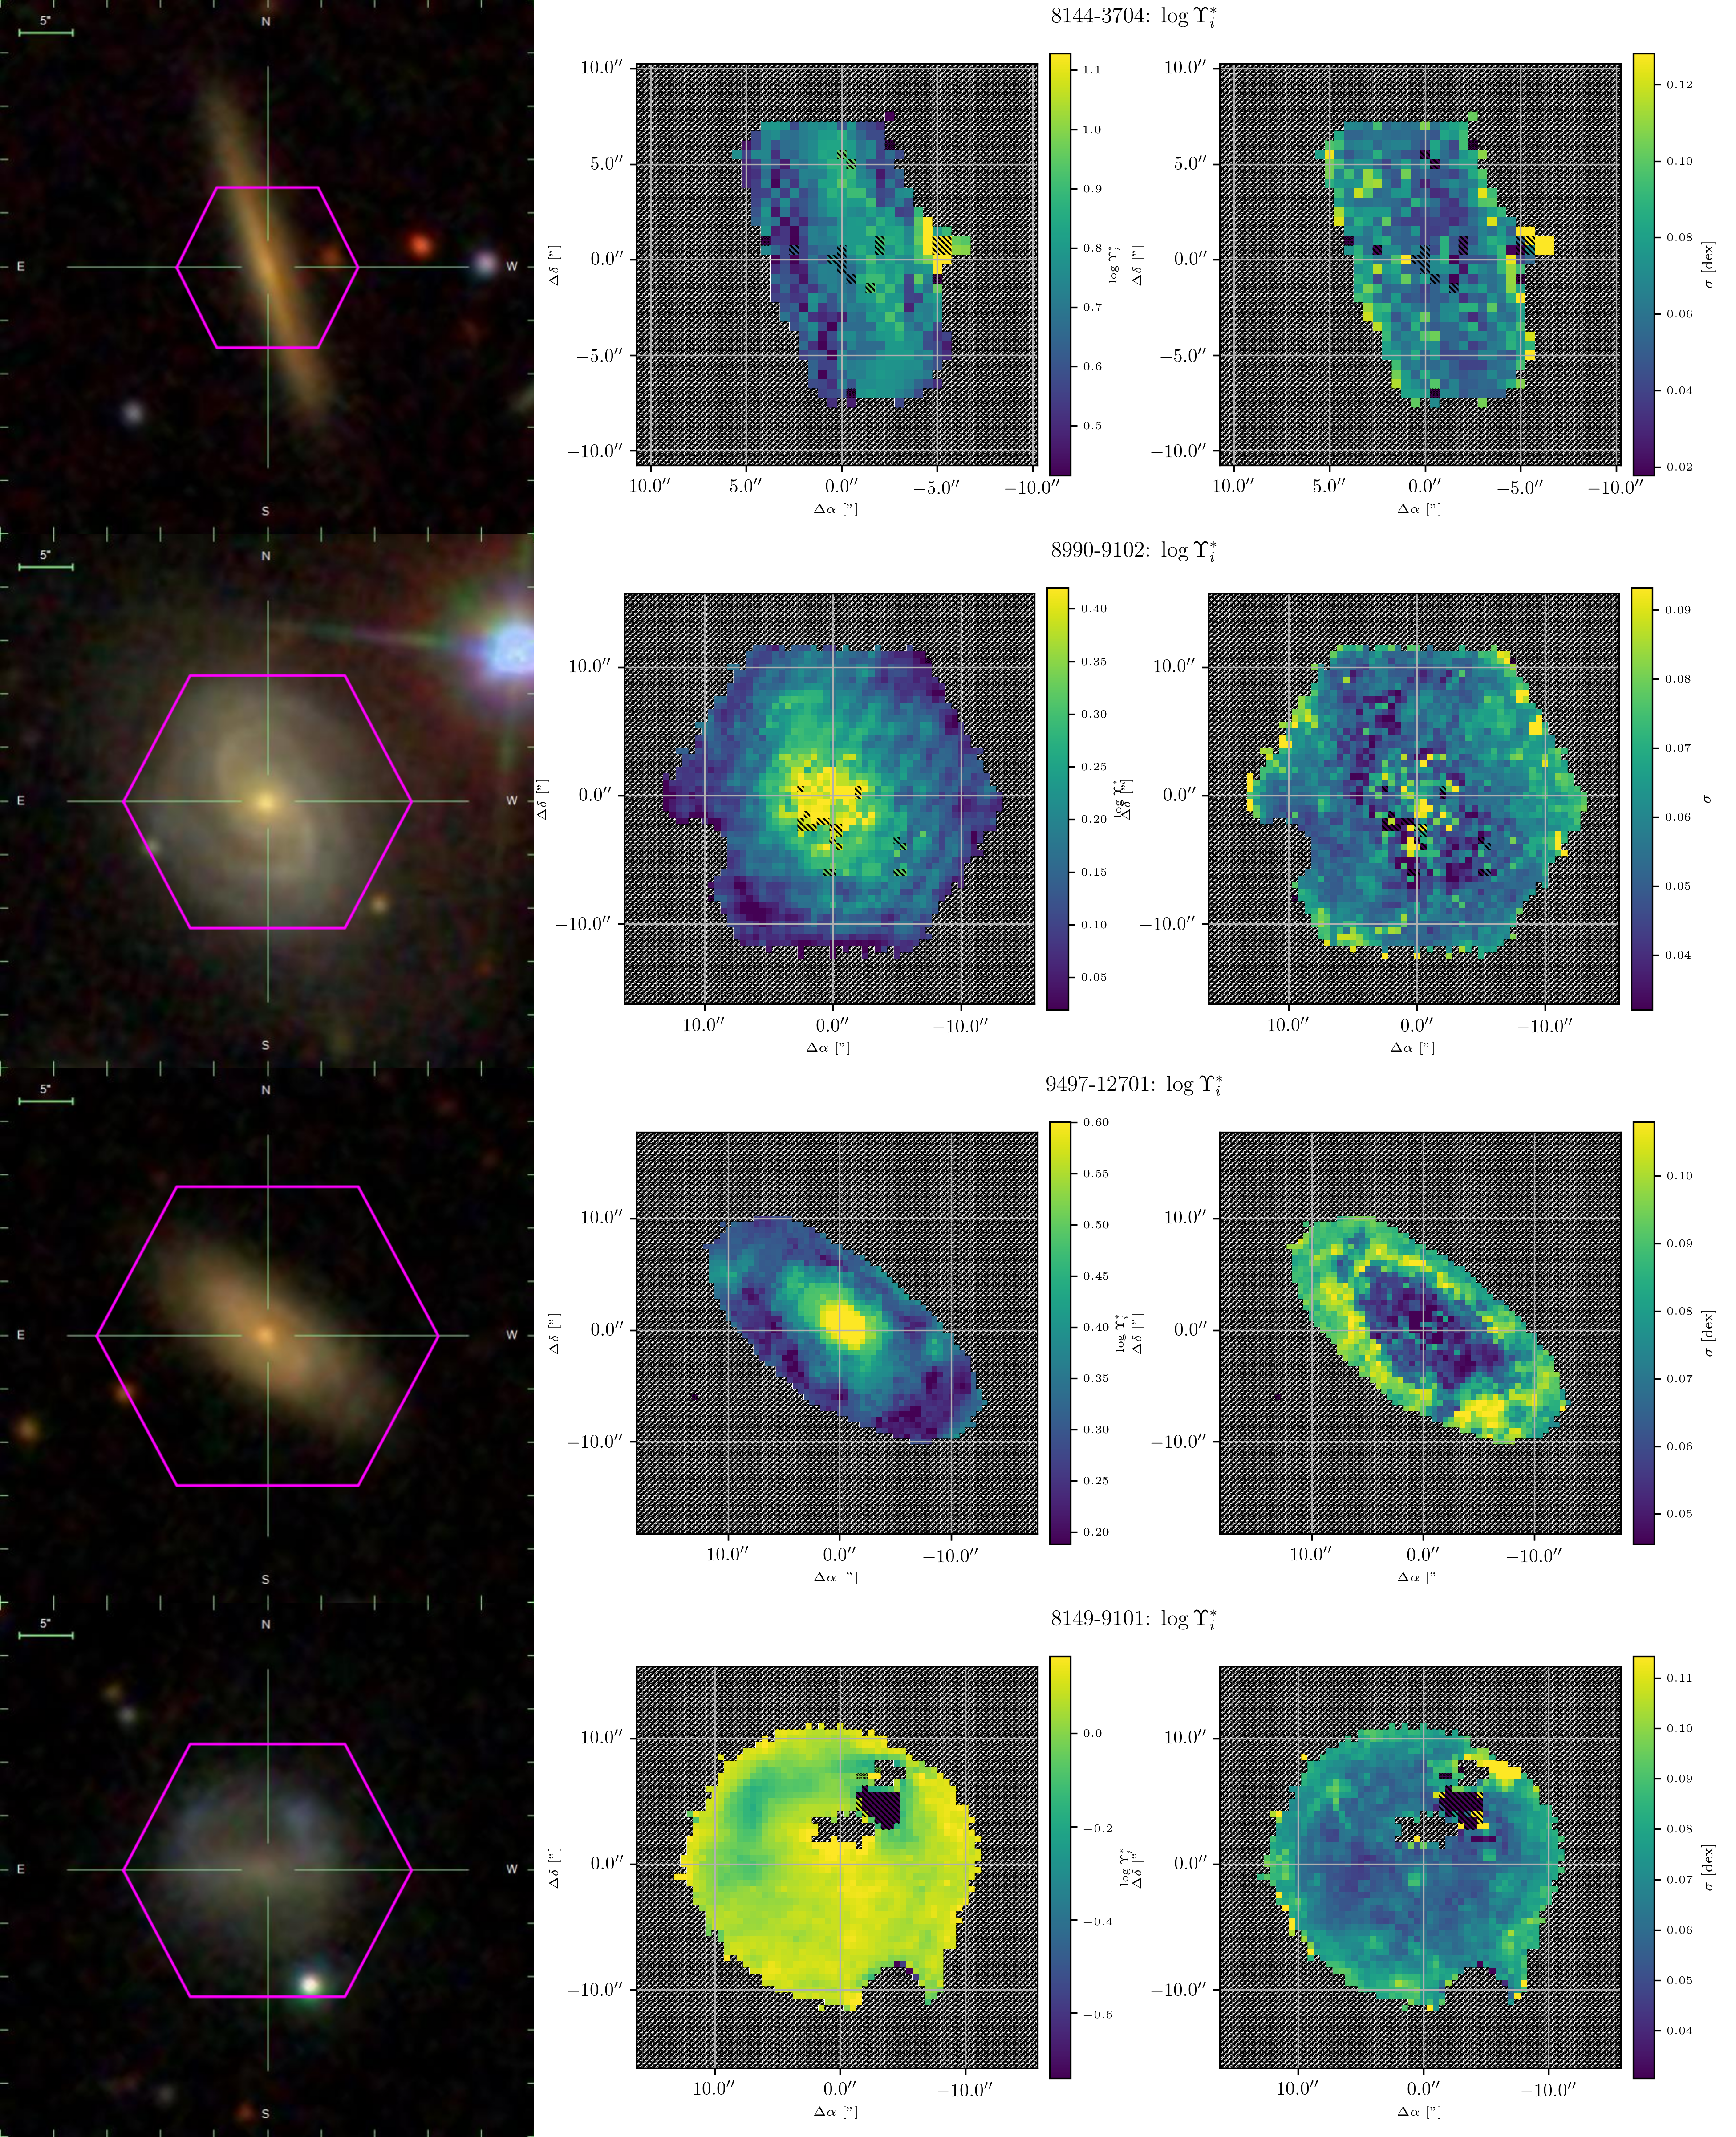
\includegraphics[width=0.95\textwidth]{LTG_montage}
    \caption[As Figure \ref{fig:ETG_montage}, but a selection of four late-type galaxies]{\fixspacing As Figure \ref{fig:ETG_montage}, but a selection of four late-type galaxies. 8114-3704 is seen edge-on \& exhibits a dust lane, 8990-9102 is star-forming and is seen nearly face-on, 9497-12701 is moderately-inclined and has a low SFR, and 8149-9101 is a low-mass dwarf galaxy with ongoing star-formation.}
    \label{fig:LTG_montage}
\end{figure*}
%
The maps of resolved stellar mass-to-light ratio are spatially smooth, suggesting that the PC down-projection of two nearby spaxels indeed reflects the PSF of the data induced by the dithering and wavelength-rectification processes: The process of assembling individual science exposures (each at one of three positions on a galaxy's face, and subject to some distinct differential atmospheric refraction, attenuation by the atmosphere, etc.) detailed in \citet[][Section 9.2]{manga_drp} induces a spatial covariance between nearby spaxels. Therefore, one might expect that two spaxels that are nearby to one another might have similar estimates of mass-to-light ratio, beyond the degree to which the underlying stellar populations are similar. We do in fact qualitatively observe this smooth variation in the resolved stellar mass-to-light ratio.

\subsection{Remaining spectral-fitting systematics and degeneracies}

The use of a synthetic stellar library represents the most uncertain systematic in this work. Perhaps most importantly, the one-dimensional stellar atmospheres adopted for this work are fixed in abundance of $\alpha$ elements. In reality, ${\rm \frac{\alpha}{Fe}}$ is known to differ from the solar value in the central regions of early-type galaxies \citep{worthey_faber_92, matteucci_94, thomas_greggio_bender_99}. These are among the brightest spaxels in the survey. Indeed, such regions are occasionally observed to have poorly-determined estimates of \logml{i} (Section \ref{chap1:subsec:data_quality}). Fortunately, the MaStar project is now undertaking bright-time observations of stars using the BOSS spectrograph, the same instrument as is used for MaNGA galaxies. A resolution- and wavelength-range-matched sample of about 10,000 stars with a wide variety of stellar parameters will represent an important value-added deliverable of MaNGA, as well as a useful input to SPS codes. Secondarily, strong constraints on the prevalence and impact of non-standard stellar evolution scenarios (such as blue stragglers and blue horizontal branch) will inform future choices of SPS inputs.

\subsection{Public Data and Future Work}
The resolved estimates of stellar mass-to-light ratio treated in detail in this work will be included in the next public data release of SDSS-IV as a value-added catalog (VAC). In \citetalias{pace_19b_pca} (next in this series), we:

\begin{itemize}
    \item Further evaluate the resolved stellar mass-to-light estimates of MaNGA galaxies by transforming them to maps of stellar mass surface density and comparing to radial averages of dynamical mass surface density from the DiskMass Survey \citep{diskmass_i}.
    \item Devise a method of aperture-correcting estimates of resolved stellar mass in order to obtain estimates of total galaxy stellar mass, which will also be released to the community.
    \item Compare the PCA-derived estimates of total galaxy stellar mass to those from integrated photometry.
    \item Evaluate the factors contributing to a mass deficit in IFU-summed spectra, relative to summing stellar masses in individual spaxels.
\end{itemize}

Also provided will be light-weight \texttt{python} scripting utilities to assist in accessing the resolved mass-to-light maps. Resolved maps of additional parameters (such as dust, SFH burst diagnostics, and stellar metallicity) may be released as part of future scientific analyses (they may also be obtained from the authors, upon request).